\documentclass[11pt]{article}
\usepackage[a4paper,left=1.5cm,right=1.5cm,top=1.5cm,bottom=1.5cm]{geometry}
\usepackage{fancyhdr}
\renewcommand{\headrulewidth}{1pt}
\fancyhead[C]{\textbf{[LINGI2132] Languages \& Translators}}
\fancyhead[L]{Assignment 2 -- Theory}
\fancyhead[R]{Group 55}

\usepackage[T1]{fontenc}
\usepackage[utf8]{inputenc}
\usepackage[english]{babel}
\usepackage{syntax}
\let\syntleft\relax
\let\syntright\relax
\setlength{\grammarindent}{3.5em}
\usepackage{graphicx}
\usepackage{subcaption}
\usepackage{mathtools,amssymb, mathrsfs,amsthm}
\usepackage[binary-units=true,separate-uncertainty = true,multi-part-units=single]{siunitx}
\usepackage{float}
\setlength{\parskip}{1ex plus 0.5ex minus 0.2ex}
\newcommand{\hsp}{\hspace{20pt}}
\newcommand{\HRule}{\rule{\linewidth}{0.5mm}}
\graphicspath{{img/}}
\usepackage{caption}
\usepackage{textcomp}
\usepackage{array}
\usepackage{color}
\usepackage{tabularx,booktabs}
\usepackage{titlesec}
\usepackage{wrapfig}
\titlespacing{\section}{0pt}{\parskip}{-\parskip}
\titlespacing{\subsection}{0pt}{\parskip}{-\parskip}
\titlespacing{\subsubsection}{0pt}{\parskip}{-\parskip}
\pagestyle{fancy}
\usepackage{minted}
\usepackage{csquotes}
\usepackage[linktoc=all]{hyperref}
\hypersetup{breaklinks=true}
\usepackage{tikz}
\usetikzlibrary{automata,positioning}
\DeclareMathOperator{\first}{first}
\DeclareMathOperator{\follow}{follow}
\newcommand{\id}{\mathrm{id}}
\newcommand{\E}{\textnormal{E}}
\newcommand{\Ep}{\textnormal{E'}}
\newcommand{\T}{\textnormal{T}}
\newcommand{\Tp}{\textnormal{T'}}
\newcommand{\F}{\textnormal{F}}
\renewcommand{\epsilon}{\varepsilon}
\renewcommand{\theta}{\vartheta}
\renewcommand{\kappa}{\varkappa}
\renewcommand{\rho}{\varrho}
\renewcommand{\phi}{\varphi}

\begin{document}
\section{Lexical Analysis}
\subsection{}
Some words in the language described by \(ab^*c^* | (ab)^*c\) are \(a\), \(ab\), \(abc\), \(abbc\), \(ababc\).

\subsection{}
The NFA obtained by applying Thompson's construction is shown on Figure~\ref{fig:thompsonnfa}.
\begin{figure}[H]
	\centering
	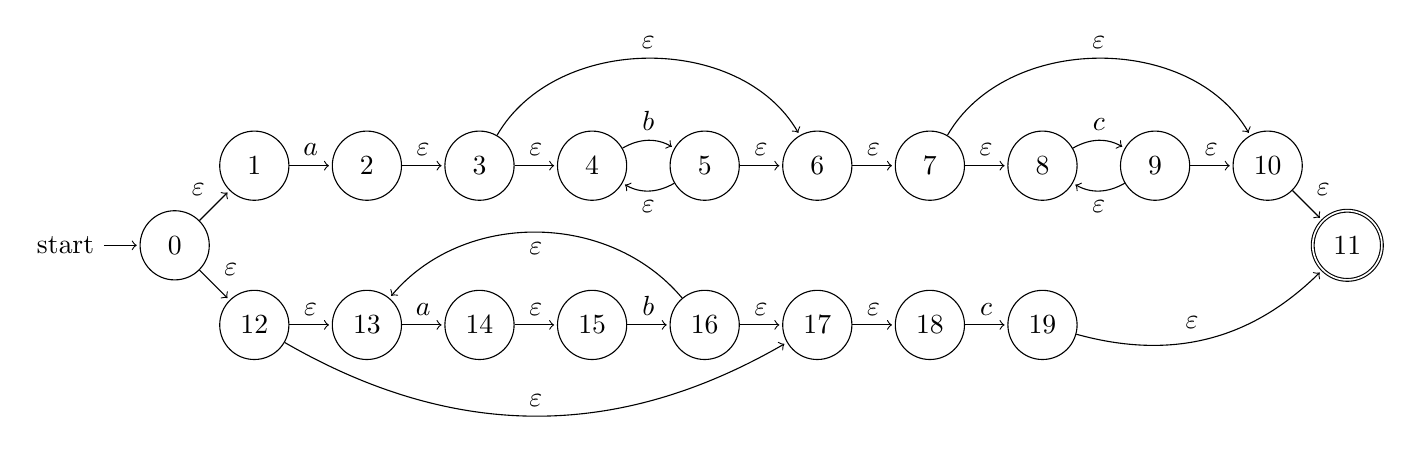
\begin{tikzpicture}[shorten >=1pt,node distance=1.43cm,on grid,auto]
	\node[state,initial] (0) {\(0\)};
	\node[state] (1) [above right=of 0] {\(1\)};
	\node[state] (2) [right=of 1] {\(2\)};
	\node[state] (3) [right=of 2] {\(3\)};
	\node[state] (4) [right=of 3] {\(4\)};
	\node[state] (5) [right=of 4] {\(5\)};
	\node[state] (6) [right=of 5] {\(6\)};
	\node[state] (7) [right=of 6] {\(7\)};
	\node[state] (8) [right=of 7] {\(8\)};
	\node[state] (9) [right=of 8] {\(9\)};
	\node[state] (10) [right=of 9] {\(10\)};
	\node[state, accepting] (11) [below right=of 10] {\(11\)};
	\node[state] (12) [below right=of 0] {\(12\)};
	\node[state] (13) [right=of 12] {\(13\)};
	\node[state] (14) [right=of 13] {\(14\)};
	\node[state] (15) [right=of 14] {\(15\)};
	\node[state] (16) [right=of 15] {\(16\)};
	\node[state] (17) [right=of 16] {\(17\)};
	\node[state] (18) [right=of 17] {\(18\)};
	\node[state] (19) [right=of 18] {\(19\)};
	\path[->]
	(0) edge node {\(\epsilon\)} (1)
	(1) edge node {\(a\)} (2)
	(2) edge node {\(\epsilon\)} (3)
	(3) edge node {\(\epsilon\)} (4)
	(4) edge [bend left] node {\(b\)} (5)
	(5) edge [bend left] node {\(\epsilon\)} (4)
	(5) edge node {\(\epsilon\)} (6)
	(3) edge [in=120, out=60] node {\(\epsilon\)} (6)
	(6) edge node {\(\epsilon\)} (7)
	(7) edge node {\(\epsilon\)} (8)
	(8) edge [bend left] node {\(c\)} (9)
	(9) edge [bend left] node {\(\epsilon\)} (8)
	(9) edge node {\(\epsilon\)} (10)
	(7) edge [in=120, out=60] node {\(\epsilon\)} (10)
	(10) edge node {\(\epsilon\)} (11)
	(0) edge node {\(\epsilon\)} (12)
	(12) edge node {\(\epsilon\)} (13)
	(13) edge node {\(a\)} (14)
	(14) edge node {\(\epsilon\)} (15)
	(15) edge node {\(b\)} (16)
	(16) edge [in=50, out=130] node {\(\epsilon\)} (13)
	(16) edge node {\(\epsilon\)} (17)
	(12) edge [bend right] node {\(\epsilon\)} (17)
	(17) edge node {\(\epsilon\)} (18)
	(18) edge node {\(c\)} (19)
	(19) edge [bend right] node {\(\epsilon\)} (11);
	\end{tikzpicture}
	\caption{Thompson construction for the regular expression \(ab^*c^* | (ab)^*c\).}
	\label{fig:thompsonnfa}
\end{figure}
\subsection{}
The NFA obtained by the Thompson construction can be transformed into a DFA by computing meta-states in the new DFA, with a transition between meta-states indicating that the NFA states corresponding to the target meta-state are reachable by applying the transition to at least on of the NFA states in the origin meta-state.
A meta-state is accepting if it contains an accepting state in the NFA.
The resulting DFA is given in Figure~\ref{fig:nfa2dfa}.
\begin{figure}[H]
	\centering
	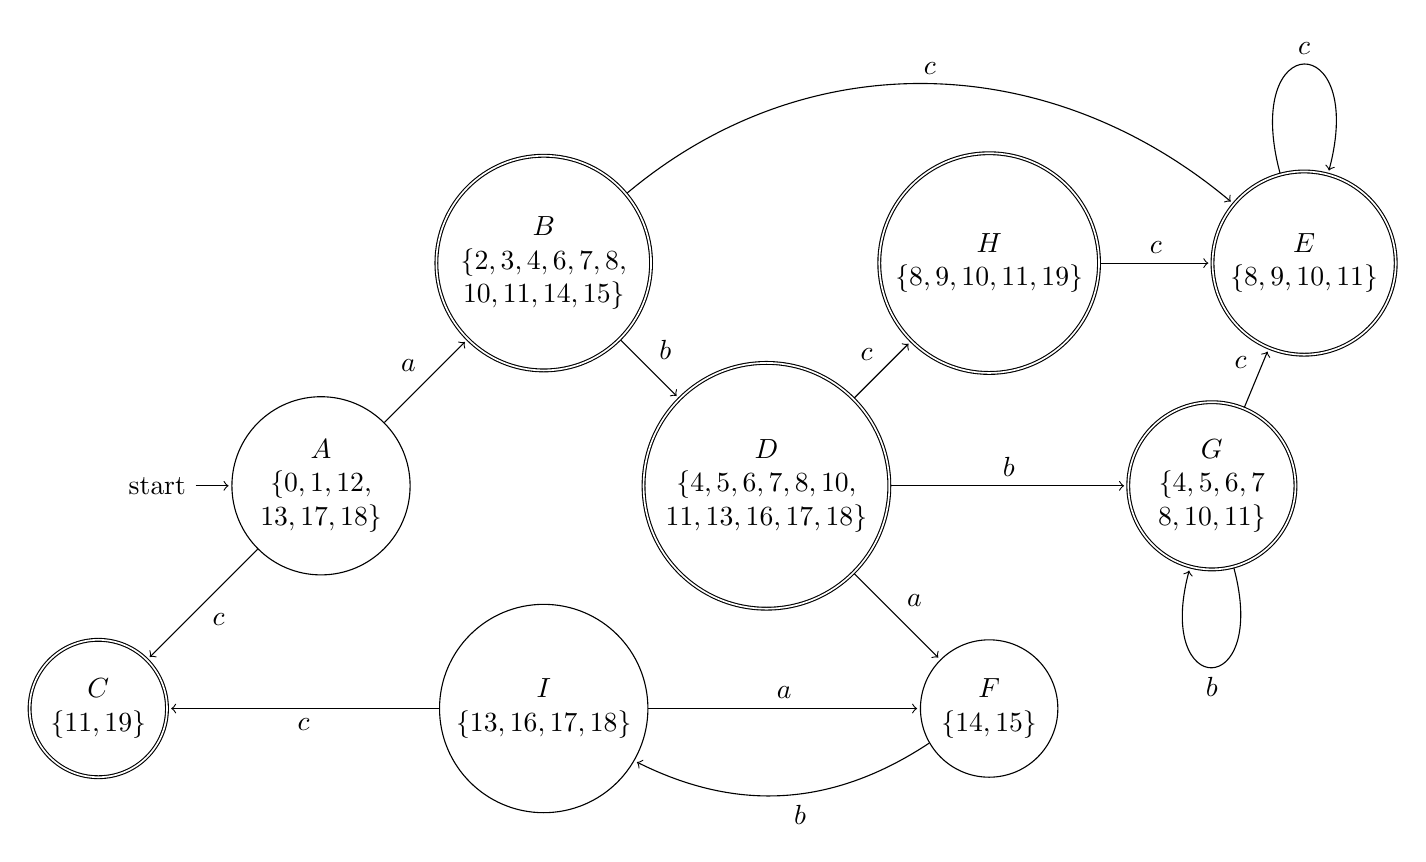
\begin{tikzpicture}[shorten >=1pt,node distance=4cm,on grid,auto]
	\node[state,initial] (A) [align=center] {\(A\) \\ \(\{0, 1, 12,\) \\ \(13, 17, 18\}\)};
	\node[state, accepting] (B) [above right=of A, align=center]  {\(B\) \\ \(\{2, 3, 4, 6, 7, 8,\) \\ \(10, 11, 14, 15\}\)};
	\node[state, accepting] (D) [below right=of B, align=center] {\(D\) \\ \(\{4, 5, 6, 7, 8, 10,\) \\ \(11, 13, 16, 17, 18\}\)};
	\node[state, accepting] (H) [above right=of D, align=center] {\(H\) \\ \(\{8, 9, 10, 11, 19\}\)};
	\node[state, accepting] (E) [right=of H, align=center] {\(E\) \\ \(\{8, 9, 10, 11\}\)};
	\node[state] (F) [below right=of D, align=center] {\(F\) \\ \(\{14, 15\}\)};
	\node[state] (I) [below left=of D, align=center] {\(I\) \\ \(\{13, 16, 17, 18\}\)};
	\node[state, accepting] (G) [above right=of F, align=center] {\(G\) \\ \(\{4, 5, 6, 7\) \\ \(8, 10, 11\}\)};
	\node[state, accepting] (C) [below left=of A, align=center] {\(C\) \\ \(\{11, 19\}\)};
	\path[->]
	(A) edge node {\(a\)} (B)
	(A) edge node {\(c\)} (C)
	(B) edge  node {\(b\)} (D)
	(B) edge [in=140, out=40] node {\(c\)} (E)
	(D) edge node {\(a\)} (F)
	(D) edge node {\(b\)} (G)
	(D) edge node {\(c\)} (H)
	(E) edge [loop above] node {\(c\)} (E)
	(F) edge [bend left] node {\(b\)} (I)
	(G) edge [loop below] node {\(b\)} (G)
	(G) edge node {\(c\)} (E)
	(H) edge node {\(c\)} (E)
	(I) edge node {\(a\)} (F)
	(I) edge node {\(c\)} (C);
	\end{tikzpicture}
	\caption{DFA corresponding to the regular expression \(ab^*c^* | (ab)^*c\), obtained by computing \(\epsilon\)-closures on the NFA obtained by Thompson's construction.}
	\label{fig:nfa2dfa}
\end{figure}
\subsection{}
The minimal DFA obtained with Hopcroft's algorithm is shown on Figure~\ref{fig:mindfa}.
For each partition, the corresponding metastate in the previous DFA is shown.
\begin{figure}[H]
	\centering
	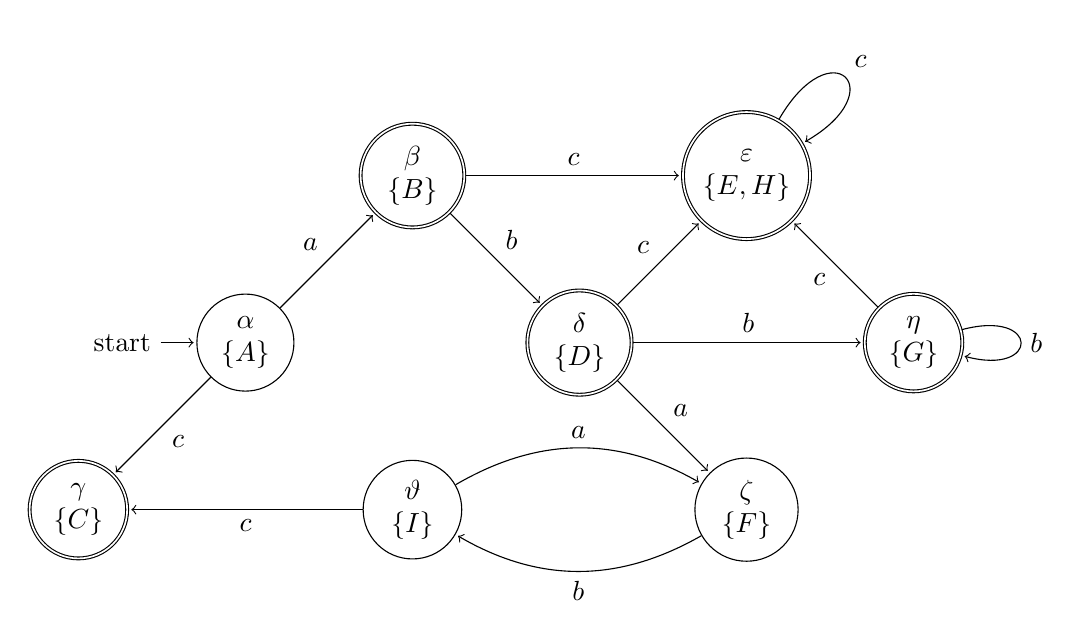
\begin{tikzpicture}[shorten >=1pt,node distance=3cm,on grid,auto]
	\node[state,initial] (alpha) [align=center] {\(\alpha\) \\ \(\{A\}\)};
	\node[state, accepting] (beta) [above right=of alpha, align=center]  {\(\beta\) \\ \(\{B\}\)};
	\node[state, accepting] (delta) [below right=of beta, align=center] {\(\delta\) \\ \(\{D\}\)};
	\node[state, accepting] (epsilon) [above right=of delta, align=center] {\(\epsilon\) \\ \(\{E, H\}\)};
	\node[state] (zeta) [below right=of delta, align=center] {\(\zeta\) \\ \(\{F\}\)};
	\node[state] (theta) [below left=of delta, align=center] {\(\theta\) \\ \(\{I\}\)};
	\node[state, accepting] (eta) [above right=of zeta, align=center] {\(\eta\) \\ \(\{G\}\)};
	\node[state, accepting] (gamma) [below left=of alpha, align=center] {\(\gamma\) \\ \(\{C\}\)};
	\path[->]
	(alpha) edge node {\(a\)} (beta)
	(alpha) edge node {\(c\)} (gamma)
	(beta) edge  node {\(b\)} (delta)
	(theta) edge node {\(c\)} (gamma)
	(theta) edge [bend left] node {\(a\)} (zeta)
	(zeta) edge [bend left] node {\(b\)} (theta)
	(beta) edge  node  {\(c\)} (epsilon)
	(delta) edge  node {\(c\)} (epsilon)
	(delta) edge node {\(a\)} (zeta)
	(delta) edge node {\(b\)} (eta)
	(eta) edge [loop right] node {\(b\)} (eta)
	(epsilon) edge [in=30,out=60, loop] node {\(c\)} (epsilon)
	(eta) edge node {\(c\)} (epsilon);
	\end{tikzpicture}
	\caption{Minimal DFA for the regular expression \(ab^*c^* | (ab)^*c\).}
	\label{fig:mindfa}
\end{figure}
\subsection{}
\textit{See code.}

\section{Parsing}
\subsection{}
\label{sec:2.1}
The given grammar is left-recursive, hence it can not be LL(\(1\)).
An equivalent LL(\(1\)) grammar is
\begin{grammar}
	<E> ::= TE'
	
	<E'> ::= \(+\)TE' | \(-\)TE' | \(\epsilon\)
	
	<T> ::= FT'
	
	<T'> ::= \(\times\)FT' | \(/\)FT' | \(\epsilon\)
	
	<F> ::= (E) | id
\end{grammar}

\subsection{}
The following First-sets and Follow-sets were computed:
\begin{align*}
\first(\E) &= \{(, \id\}, \\
\first(\Ep) &= \{+, -, \epsilon\}, \\
\first(\T) &= \{(, \id\}, \\
\first(\Tp) &= \{\times, /, \epsilon\}, \\
\first(\F) &= \{(, \id\}, \\
\follow(\E) &= \{\#, )\}, \\
\follow(\Ep) &= \{\#, )\}, \\
\follow(\T) &= \{(+, -, \#, )\}, \\
\follow(\Tp) &= \{+, -, \#, )\}, \\
\follow(\F) &= \{+, -, \times, /, \#, )\}.
\end{align*}

The parsing table for the LL(\(1\)) grammar is given in Table~\ref{tab:parsing}.
\begin{table}[H]
	\centering
	\begin{tabular}{l|cccccccc}
		\toprule
		 & \(+\) & \(-\) & \(\times\) & \(/\) & ( & ) & \(\id\) & \# \\
		\midrule
		E & & & & & 1 & & 1 & \\
		E' & 2 & 3 & & & & 4 & & 4 \\
		T & & & & & 5 & & 5 & \\
		T' & 8 & 8 & 6 & 7 & & 8 & & 8 \\
		F & & & & & 9 & & 10 & \\
		\bottomrule
	\end{tabular}
	\caption{Parsing table for the LL(\(1\)) grammar given in Section~\ref{sec:2.1}.}
	\label{tab:parsing}
\end{table}
\subsection{}
Table~\ref{tab:exec} shows the steps in parsing \(\id + (\id \times \id - \id / \id)\).
\begin{table}[H]
	\[
	\begin{array}{lrc}
		\toprule
		 \multicolumn{1}{c}{\textnormal{Stack}} & \multicolumn{1}{c}{\textnormal{Input}} & \textnormal{Output} \\
		\midrule
		\# \E & \id + (\id \times \id - \id / \id) \# & \\
		\# \Ep \T & \id + (\id \times \id - \id / \id) \# & 1 \\
		\# \Ep \Tp \F & \id + (\id \times \id - \id / \id) \# & 5 \\
		\# \Ep \Tp \id & \id + (\id \times \id - \id / \id) \# & 10 \\
		\# \Ep \Tp & + (\id \times \id - \id / \id) \# & \\
		\# \Ep & + (\id \times \id - \id / \id) \# & 8 \\
		\# \Ep \T + & + (\id \times \id - \id / \id) \# & 2 \\
		\# \Ep \T & (\id \times \id - \id / \id) \# & \\
		\# \Ep \Tp \F & (\id \times \id - \id / \id) \# & 5 \\
		\# \Ep \Tp )\E( & (\id \times \id - \id / \id) \# & 9 \\
		\# \Ep \Tp )\E & \id \times \id - \id / \id) \# & \\
		\# \Ep \Tp )\Ep \T & \id \times \id - \id / \id) \# & 1 \\
		\# \Ep \Tp )\Ep \Tp \F & \id \times \id - \id / \id) \# & 5 \\
		\# \Ep \Tp )\Ep \Tp \id & \id \times \id - \id / \id) \# & 10 \\ 
		\# \Ep \Tp )\Ep \Tp & \times \id - \id / \id) \# & \\
		\# \Ep \Tp )\Ep \Tp \F \times & \times \id - \id / \id) \# & 6 \\
		\# \Ep \Tp )\Ep \Tp \F & \id - \id / \id) \# & \\
		\# \Ep \Tp )\Ep \Tp \id & \id - \id / \id) \# & 10 \\
		\# \Ep \Tp )\Ep \Tp & - \id / \id) \# & \\
		\# \Ep \Tp )\Ep & - \id / \id) \# & 8 \\
		\# \Ep \Tp )\Ep \T - & - \id / \id) \# & 3 \\
		\# \Ep \Tp )\Ep \T & \id / \id) \# & \\
		\# \Ep \Tp )\Ep \Tp \F & \id / \id) \# & 5 \\
		\# \Ep \Tp )\Ep \Tp \id & \id / \id) \# & 10 \\
		\# \Ep \Tp )\Ep \Tp & / \id) \# & \\
		\# \Ep \Tp )\Ep \Tp \F / & / \id) \# & 7 \\
		\# \Ep \Tp )\Ep \Tp \F & \id) \# & \\
		\# \Ep \Tp )\Ep \Tp \id & \id) \# & 10 \\
		\# \Ep \Tp )\Ep \Tp & ) \# & \\
		\# \Ep \Tp )\Ep & ) \# & 8 \\
		\# \Ep \Tp ) & ) \# & 4 \\
		\# \Ep \Tp & \# & \\
		\# \Ep & \# & 8 \\
		\# & \# & 4 \\
		\bottomrule
	\end{array}
	\]
	\caption{Example of parsing \(\id + (\id \times \id - \id / \id)\).}
	\label{tab:exec}
\end{table}

\section{DFA}
Yes, a DFA can accept an infinite language.
One can prove that a DFA \(\mathscr{D}\) with \(n\) states accepts an infinite language if and only if \(\mathscr{D}\) accepts a string of length \(k\), where \(n \le k < 2n\).
One example is the language \(L(a^*)\), which has an infinite number of strings in it, but is accepted by the DFA in Figure~\ref{fig:infinitedfa}.
Unsurprisingly, the property above is verified for this DFA.
\begin{figure}[H]
	\centering
	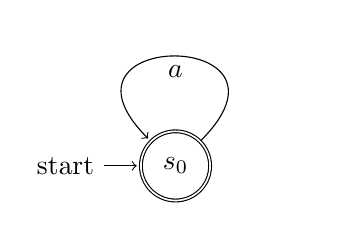
\begin{tikzpicture}[shorten >=1pt,node distance=4cm,on grid,auto]
	\node[state,initial, accepting] (q) {\(s_0\)};
	\path[->]
	(q) [loop] edge node {$a$} (q);
	\end{tikzpicture}
	\caption{DFA which accepts the infinite language \(L(a^*)\).}
	\label{fig:infinitedfa}
\end{figure}
This is a theoretical result, however.
In practice, detecting cycles which contain a start state and a final state is a more efficient way of determining whether a DFA accepts an infinite language.
This can be done using depth-first search.

\section{Language}
This language is not regular.
\begin{proof}
	Let \(L\) be the language of well-balanced parentheses.
	By contradiction, assume that \(L\) is regular.
	By the pumping lemma, there exists some constant \(p\) such that any word \(w\) of length at least \(p\) in \(L\) can be split into \(w = xyz\) such that
	\begin{itemize}
		\item \(|xy| \le p\);
		\item \(|y| > 0\);
		\item \(x y^i z \in L\) for all \(i \ge 0\).
	\end{itemize}
	
	Take \(w\) to be the balanced string consisting of \(p\) left parentheses followed by \(p\) right parentheses.
	The first condition of the pumping lemma then gives that \(y\) consists only of left parentheses, while the second guarantees \(y\) is nonempty.
	By the third condition, \(xyyz\) should also be part of \(L\).
	However, this is not the case, since by construction \(xyyz\) contains more left parentheses than right parentheses. The initial assumption that \(L\) is regular must thus be false.
\end{proof}
\end{document}